%!TEX root = /Users/jakubkonka/Thesis/Thesis.tex
\chapter{Py3k Discrete-Event System Simulator}
\label{cha:py3k_discrete_event_system_simulator}

\minitoc
\vspace{10mm}

The discrete-event system (DES) simulation study outlined in Chapter~\ref{cha:dynamics_of_network_selection_in_the_digital_marketplace} was conducted using software that was developed during this research from scratch in Python programming language, version 3 (Py3k). Py3k was chosen mainly due to the fact that it is a dynamically-typed language which makes prototyping quicker than in a statically-typed language such as C++. This allows the researcher to focus more on the design and results of the experiment rather than its implementation. Furthermore, Py3k features a set of libraries that further simplify the implementation stage of the DES simulation; for example, \lstinline{subprocess} module allows the execution of multiple simulation runs in parallel~\cite{Py3kSubprocess}, while \lstinline{numpy}, \lstinline{scipy}, and \lstinline{matplotlib} modules provide a set of convenience routines for numerical computation and scientific plotting in Py3k~\cite{Numpy, Scipy, Matplotlib}. On the other hand, since Py3k is an interpreted language, it can potentially be slower in execution time and less memory efficient than a compiled language such as C++~\cite{Py3kC++}; however, it does not visibly increase the overall cost of the simulation study since the computer resources are inexpensive.

The software is released under the MIT License, and is available for download on Github: \url{https://github.com/kubkon/des-in-python}.

\section{Description of the Simulator}
\label{sec:description_of_the_simulator_simappendix}

\subsection{High-level Overview}
\label{sub:high_level_overview_simappendix}
The simulator is composed of four building blocks: \lstinline{SimulationEngine} class, \lstinline{EventHandler} class, \lstinline{Event} class, and \lstinline{PRNG} class. The \lstinline{SimulationEngine} class provides all the core functionality of a DES simulator. It advances the simulation time, and implements the event list. The \lstinline{EventHandler} class is an abstract base class (or an interface), and provides an outline of the basic functionality that any proper subclass must implement. In general, it is responsible for generating and handling simulation specific events; for example, customer arrival and departure events in a simulation of an M/M/1 queue. The \lstinline{Event} class implements basic structure of a generic event used by the simulator. Finally, the \lstinline{PRNG} class provides basic pseudo-random number generation (PRNG) routines, and currently, it is a wrapper class for the Py3k \lstinline{random} module.

\begin{figure}[t]
  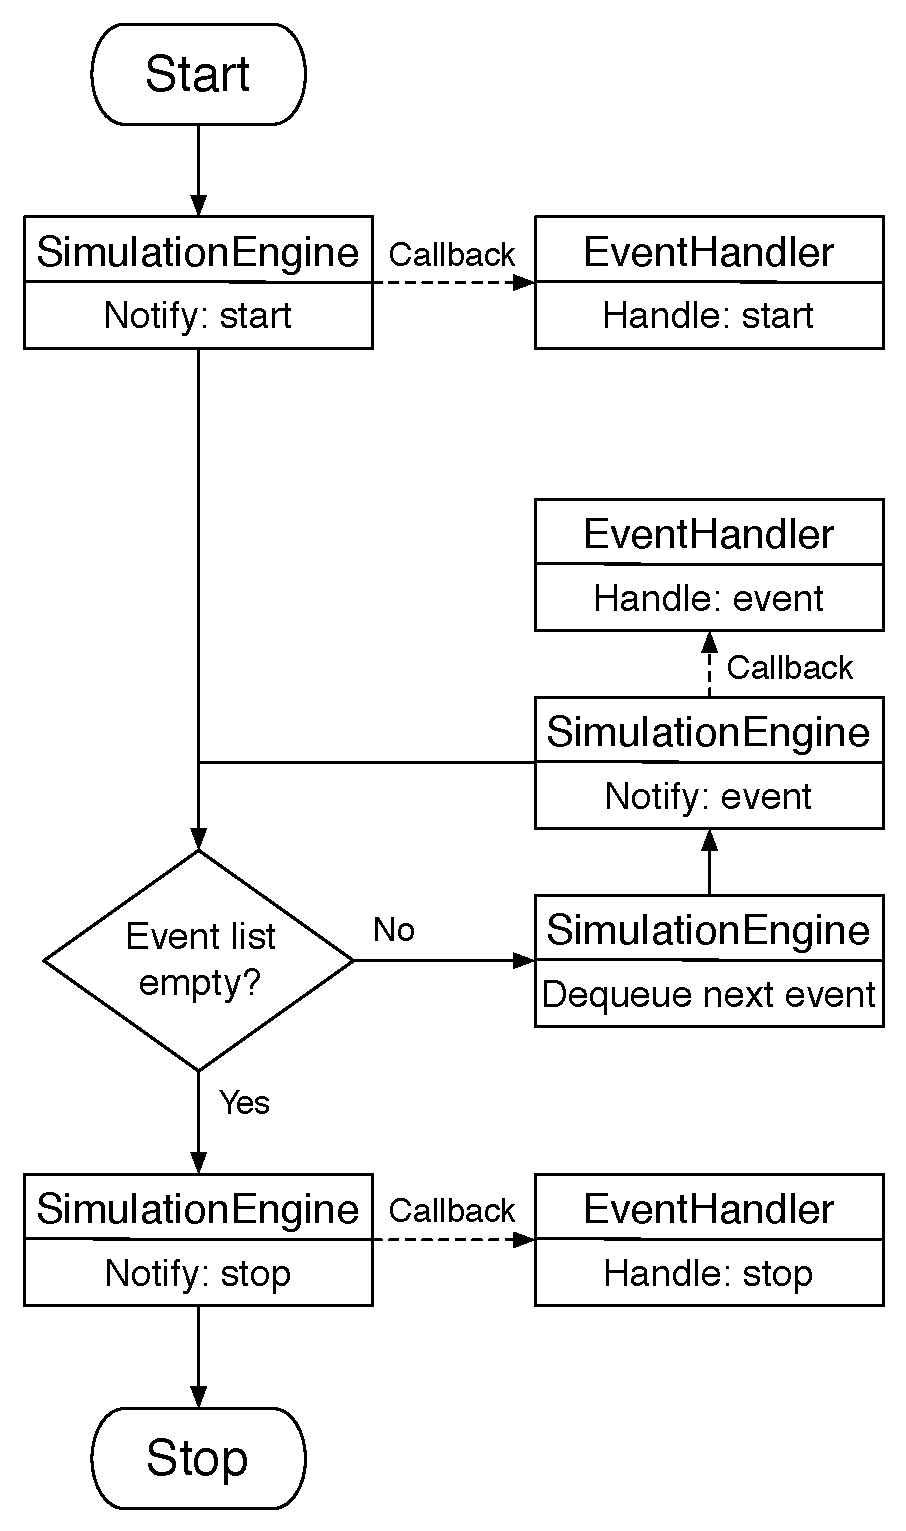
\includegraphics[width=3in]{Appendices/Figures/simulation_flow}
  \caption{Simplified simulation flow}
  \label{fig:simulation_flow_simappendix}
\end{figure}

Figure~\ref{fig:simulation_flow_simappendix} depicts the simplified flow of the simulation. Upon the start of the simulation, a \lstinline{SimulationEngine} class instance notifies an \lstinline{EventHandler} class instance\footnote{Technically, a \lstinline{SimulationEngine} class instance notifies an instance of a class that subclasses the \lstinline{EventHandler} class; however, to keep the description simple and generic, we shall refer to it as an \lstinline{EventHandler} class instance.} of the start of the simulation (via a callback mechanism). At this point, the \lstinline{EventHandler} class instance should handle it by generating the first event, and passing it to the \lstinline{SimulationEngine} class instance for scheduling. Afterwards, the \lstinline{SimulationEngine} class instance dequeues the next event from the event list, and passes it to the \lstinline{EventHandler} class instance, which should update statistics related to the passed in event, and generate additional events. The process is repeated until there are no events in the event list. When the list becomes empty, the \lstinline{SimulationEngine} class instance notifies the \lstinline{EventHandler} class instance of the stop of the simulation. At this point, the \lstinline{EventHandler} class instance should save/finalize all the statistics relevant to the simulation for further processing and analysis.

\subsection{SimulationEngine Class}
\label{sub:simulationengine_class_simappendix}
As briefly mentioned in Section~\ref{sub:high_level_overview_simappendix}, the \lstinline{SimulationEngine} class provides all the core functionality of a DES simulator. In particular, the class defines the following properties:
\begin{itemize}
  \item \lstinline{self.simulation_time} stores the current simulation time. The simulation time is assumed to be in seconds; thus, \lstinline{self.simulation_time = 1} is equivalent to setting the simulation time to 1 second.
  \item \lstinline{self.prng} stores a reference to a PRNG. By default, \lstinline{self.prng = PRNG()}; that is, it references an instance of the \lstinline{PRNG} class.
  \item \lstinline{self.event_handler} stores a reference to an event handler; i.e., an instance of a class that subclasses the \lstinline{EventHandler} class. If \lstinline{self.event_handler} is unassigned in the main simulation script, then an exception is raised.
\end{itemize}

The basic use of the \lstinline{SimulationEngine} class in the main simulation script is depicted in Listing~\ref{listing:excerpt_from_main_simulation_script_simappendix}. In the listing, it is assumed that the definition of the \lstinline{SimulationEngine} class resides in the \lstinline{sim} module which, in turn, is part of the \lstinline{modules} subpackage of the \lstinline{simulator} package (line 1, Listing~\ref{listing:excerpt_from_main_simulation_script_simappendix}). Furthermore, it is assumed that \lstinline{event_handler} variable was defined somewhere else in the script, and that it is an instance of a class that subclasses the \lstinline{EventHandler} class (line 9).
\begin{lstlisting}[caption=Excerpt from main simulation script, label=listing:excerpt_from_main_simulation_script_simappendix]
import simulator.modules.sim as sim

...

### Initialize
# Create new simulation engine
se = sim.SimulationEngine()
# Attach event handler to the simulation engine
se.event_handler = event_handler

### Simulate
# Schedule finishing event at 100s
se.stop(100)
# Start simulating
se.start()
\end{lstlisting}
The simulation is started by calling the \lstinline{start()} member method of the \lstinline{SimulationEngine} class (line 15). However, it is necessary to call the \lstinline{stop(finish_time)} member method beforehand in order to specify the duration of the simulation (line 13).

Listing~\ref{listing:stop_member_method_simulationengine_simappendix} depicts the implementation of the \lstinline{stop(finish_time)} member method, while Listing~\ref{listing:start_member_method_simulationengine_simappendix} presents the implementation of the \lstinline{start()} member method. The \lstinline{stop(finish_time)} method takes one argument, \lstinline{finish_time}, which represents the finish time (or the duration) of the simulation, and schedules an end event (i.e., appends it to the event list, \lstinline{self._event_list}) with time property set to \lstinline{finish_time} (line 13, Listing~\ref{listing:stop_member_method_simulationengine_simappendix}). The end event is only scheduled if the method was not called in the past, which is verified by checking the state of the flag member variable \lstinline{self._finish_event_exists} (line 9).

\begin{lstlisting}[caption=\lstinline{stop(finish_time)} member method of the \lstinline{SimulationEngine} class, label=listing:stop_member_method_simulationengine_simappendix]
def stop(self, finish_time):
  """
  Schedules finishing event

  Arguments:
  finish_time -- Time of occurrence of the finishing event
  """
  # Check if finishing event already scheduled
  if not self._finish_event_exists:
    # Set finish time
    self._finish_time = finish_time
    # Schedule finishing event
    self._event_list += [Event(self.END_EVENT, self._finish_time)]
    self._finish_event_exists = True
\end{lstlisting}

The \lstinline{start()} method does not take any arguments, and is responsible for running the simulation in accordance with the flow chart depicted in Figure~\ref{fig:simulation_flow_simappendix}. Therefore, firstly, a check is made whether \lstinline{self.event_handler} property was assigned; failure generates an error in the form of an exception (lines 6-7, Listing~\ref{listing:start_member_method_simulationengine_simappendix}). Next, the method notifies all interested parties (usually instances of classes subclassing the EventHandler class) of the start of the simulation (line 10). The method then traverses the event list, \lstinline{self._event_list}, until it is empty (line 12). The traversal process consists of 3 steps: 1) dequeueing the most recent (imminent) event from the event list (line 14), 2) advancing the simulation time to the time of the dequeued event (line 16), and 3) notifying all interested parties of the dequeued event (line 18). Finally, when the traversal process finishes (i.e., when the event list becomes empty), the method notifies all interested parties of the stop of the simulation (line 20).

\begin{lstlisting}[caption=\lstinline{start()} member method of the \lstinline{SimulationEngine} class, label=listing:start_member_method_simulationengine_simappendix]
def start(self):
  """
  Starts simulation
  """
  # Check if an event handler is attached; if not, throw an error
  if not self.event_handler:
    raise Exception("No EventHandler attached!")
  # Notify of the start of the simulation; event handlers should
  # generate first event
  self._notify_start()
  # Traverse the event list
  while len(self._event_list) > 0:
    # Remove the imminent event from the event list
    imminent = self._event_list.pop()
    # Advance clock to the imminent event
    self.simulation_time = imminent.time
    # Notify of the current event
    self._notify_event(imminent)
  # Notify of the end of the simulation
  self._notify_stop()
\end{lstlisting}

The \lstinline{SimulationEngine} class facilitates scheduling/adding of new events to the event list via the \lstinline{schedule(event)} member method. The implementation of this method is depicted in Listing~\ref{listing:schedule_member_method_simulationengine_simappendix}. The method takes one argument, \lstinline{event}, which is an instance of the \lstinline{Event} class and represents the event that is to be appended to the event list. Before the event is appended to event list, however, the method verifies that the event is not intended to be triggered after the scheduled simulation time (line 9, Listing~\ref{listing:schedule_member_method_simulationengine_simappendix}); otherwise, the event is discarded. If the test is successful, the event is appended to the event list, \lstinline{self._event_list} (line 11). Afterwards, the event list is re-sorted based on time of occurrence of each event in a descending manner (lines 13-14). This ensures that whenever a new event is added to the list, the elements in the list are totally ordered in a last-in first-out (LIFO) style.

\begin{lstlisting}[caption=\lstinline{schedule(event)} member method of the \lstinline{SimulationEngine} class, label=listing:schedule_member_method_simulationengine_simappendix]
def schedule(self, event):
  """
  Schedules event (adds it to event list)

  Arguments:
  event -- Event to be scheduled
  """
  # Discard new event if happens after the finishing event
  if event.time < self._finish_time:
    # Add the event to the event list
    self._event_list += [event]
    # Sort the list in a LIFO style
    self._event_list.sort(key=lambda x: x.time)
    self._event_list.reverse()
\end{lstlisting}

Lastly, as shown in Listing~\ref{listing:start_member_method_simulationengine_simappendix}, the \lstinline{SimulationEngine} class facilitates 3 types of notifications: start of the simulation (via \lstinline{self._notify_start()} method), stop of the simulation (via \lstinline{self._notify_stop()} method), and notification of an event (via \lstinline{self._notify_event(event)} method). In order for an instance of a custom class to receive one of these notifications, it needs to register with the \lstinline{SimulationEngine} class. This functionality is provided by the \lstinline{register_callback(func, ttype)} method. The implementation of this method is shown in Listing~\ref{listing:register_callback_method_simulationengine_simappendix}.
\begin{lstlisting}[caption=\lstinline{register_callback(func, ttype)} member method of the \lstinline{SimulationEngine} class, label=listing:register_callback_method_simulationengine_simappendix]
def register_callback(self, func, ttype):
  """
  Register function for callback when simulation ends
  
  Arguments:
  func -- Function to call back
  ttype -- Type of the callback
  """
  self._callback_dict[ttype] += [func]
\end{lstlisting}
The method takes two arguments: \lstinline{func}, a function to invoke when the notification is due, and \lstinline{ttype}, the type of the notification which has to assume one of the following values: \lstinline{SimulationEngine.START_CALLBACK} for the start of the simulation notification, \lstinline{SimulationEngine.STOP_CALLBACK} for the stop of the simulation notification, and \lstinline{SimulationEngine.EVENT_CALLBACK} for the notification of an event. Therefore, an instance \lstinline{an_instance} of a custom class wanting to receive notifications of an event would have the following form:
\begin{lstlisting}[nolol,frame=none,numbers=none]
se.register_callback(an_instance.handle_event,
                     SimulationEngine.EVENT_CALLBACK)
\end{lstlisting}
where \lstinline{se} is assumed to be an instance of the \lstinline{SimulationEngine} class, and it is assumed that the instance \lstinline{an_instance} implements method \lstinline{self.handle_event(event)}.

\subsection{EventHandler Class}
\label{sub:eventhandler_class_simappendix}
The \lstinline{EventHandler} class provides an interface for handling events. In Python terminology, this type of a class is known as an abstract base class, and as such, it is largely devoid of any implementation; rather, it leaves the implementation of the specified member methods to its subclasses.

The class provides three abstract member methods that need to be implemented by the subclass: \lstinline{self._handle_start()}, \lstinline{self._handle_stop()}, and \lstinline{self._handle_event(event)}. The implementation of the \lstinline{self._handle_start()} method should provide a routine for handling the start of a simulation (cf. line 10, Listing~\ref{listing:start_member_method_simulationengine_simappendix}). Therefore, at the very least, it should generate the first event specific to the simulation; e.g., the first arrival event in a simulation of an M/M/1 queue. The implementation of the \lstinline{self._handle_stop()} method, on the other hand, should provide a routine for handling the stop of a simulation (cf. line 20, Listing~\ref{listing:start_member_method_simulationengine_simappendix}). For example, it could save gathered statistics to a file. Finally, the implementation of the \lstinline{self._handle_event(event)} method should provide a routine for handling the imminent event, \lstinline{event}, that was dequeued from the event list by the \lstinline{SimulationEngine} instance (cf. line 18, Listing~\ref{listing:start_member_method_simulationengine_simappendix}). Furthermore, it is expected that further generation of events specific to the simulation is performed within this method; e.g., generation of subsequent arrival events in a simulation of an M/M/1 queue.

The constructor method of the \lstinline{EventHandler} class, which is depicted in Listing~\ref{listing:init_method_eventhandler_simappendix}, expects one argument: \lstinline{simulation_engine}, a reference to a \lstinline{SimulationEngine} class instance. The reference is stored for later use by any of the \lstinline{EventHandler} class subclasses via the member variable \lstinline{self._simulation_engine} (line 9, Listing~\ref{listing:init_method_eventhandler_simappendix}). Furthermore, the constructor method of the \lstinline{EventHandler} class uses the reference to register the class (and through the properties of inheritance, any of its subclasses) to receive the notifications provided by the \lstinline{SimulationEngine} class (lines 10-19).
\begin{lstlisting}[caption=\lstinline{__init__(simulation_engine)} member method of the \lstinline{EventHandler} class, label=listing:init_method_eventhandler_simappendix]
def __init__(self, simulation_engine):
  """
  Constructs EventHandler object

  Arguments:
  simulation_engine = SimulationEngine instance
  """
  # Connect with SimulationEngine
  self._simulation_engine = simulation_engine
  # Register callback functions:
  # start of the simulation
  self._simulation_engine.register_callback(self._handle_start,
    SimulationEngine.START_CALLBACK)
  # stop of the simulation
  self._simulation_engine.register_callback(self._handle_stop,
    SimulationEngine.STOP_CALLBACK)
  # imminent event
  self._simulation_engine.register_callback(self._handle_event,
    SimulationEngine.EVENT_CALLBACK)
\end{lstlisting}

\subsection{Event Class}
\label{sub:event_class_simappendix}

\begin{lstlisting}[caption=\lstinline{__init__(identifier, time, **kwargs)} member method of the \lstinline{Event} class, label=listing:init_method_event_simappendix]
def __init__(self, identifier, time, **kwargs):
  """
  Constructs Event instance
  
  Arguments:
  identifier -- ID/type of this event
  time -- Time of occurring of this event

  Keyword arguments:
  kwargs -- Optional keyword arguments
  """
  self._identifier = identifier
  self._time = time
  self._kwargs = kwargs
\end{lstlisting}

\subsection{PRNG Class}
\label{sub:prng_class_simappendix}

\section{Validation of the Simulator}
\label{sec:validation_of_the_simulator_simappendix}
Since the simulation engine is not part of any known simulation package and was written from scratch, it should be validated prior to conducting any complex simulation study. To this end, the validation stage comprises simulation of a simple first-in first-out (FIFO) network link modeled as an M/M/1 queue, and analysis of steady-state average packet delay in the system (Figure~\ref{fig:mm1_queue_simappendix}). The M/M/1 queue was chosen since it is simple to implement, and the simulation results can directly be verified by comparison with the theoretical prediction.

\begin{figure}[t]
	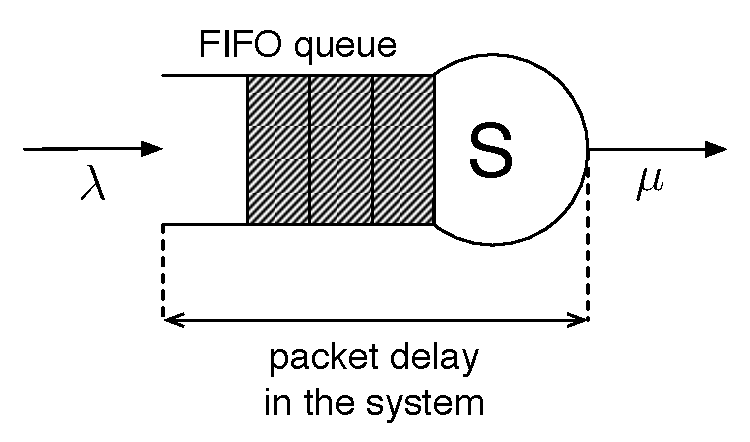
\includegraphics[width=3in]{Appendices/Figures/mm1_queue}
	\caption{Illustration of M/M/1 queuing model}
	\label{fig:mm1_queue_simappendix}
\end{figure}

\subsection{MM1EventHandler Class}
\label{sub:mm1eventhandler_class_simappendix}

\subsection{Simulation Results and Analysis}
\label{sub:simulation_results_and_analysis_simappendix}
As a quick reminder of basic queueing theory, M/M/1 queue denotes a single-server queueing system with exponential interarrival times and service times, and a FIFO queue discipline. For a proper, more in-depth treatment of queueing theory, see for example~\cite{CassandrasLafortune2008}. Let $\lambda\in\mathbb{Z}_+$ denote the mean interarrival rate, and let $\mu\in\mathbb{Z}_+$ denote the mean service rate such that $0 \le \lambda < \mu$. The steady-state mean packet delay in an M/M/1 queueing system can thus be defined as follows
\begin{equation}
	\label{eq:mm1_mean_packet_delay_simappendix}
	T = \frac{1}{\mu - \lambda},\quad T\in\displaystyle\left[\frac{1}{\mu}, \infty\right).
\end{equation}
Let $\rho = \displaystyle\frac{\lambda}{\mu}$ denote the mean link (or system) utilization. Clearly, $\rho\in [0,1)$. Hence, the steady-state mean packet delay in Equation~\eqref{eq:mm1_mean_packet_delay_simappendix} can be rewritten as
\begin{equation}
	\label{eq:mm1_mean_packet_delay_2_simappendix}
	T(\rho) = \frac{1}{\mu(1 - \rho)}.
\end{equation}

\begin{table}[p!]
	\caption{Simulation estimated M/M/1 queue steady-state average packet delay}
	\begin{tabular*}{0.5\columnwidth}[L]{@{\extracolsep{\fill}}c c c}
		\hlx{vhv}
		\textbf{Average} & \multicolumn{2}{c}{\textbf{Average packet delay, s}} \\
		\textbf{link utilization} & Mean & $95\%$ confidence interval (x $10^{-5}$) \\
		\hlx{vhv}
		 $0.1$	& $0.02224$	& $4.38835$\\
		 $0.2$	& $0.02497$	& $3.88310$\\
		 $0.3$	& $0.02858$	& $4.32400$\\
		 $0.4$	& $0.03333$	& $6.22518$\\
		 $0.5$	& $0.03999$	& $7.67952$\\
		 $0.6$	& $0.04997$	& $13.62042$\\
		 $0.7$	& $0.06654$	& $22.25786$\\
		 $0.8$	&	$0.10025$	& $51.73063$\\
		 $0.9$	& $0.20100$	& $192.24667$\\
		 \hlx{vhs}
	\end{tabular*}
	\label{tab:mm1_simulation_results_simappendix}
\end{table}
\begin{figure}[p!]
	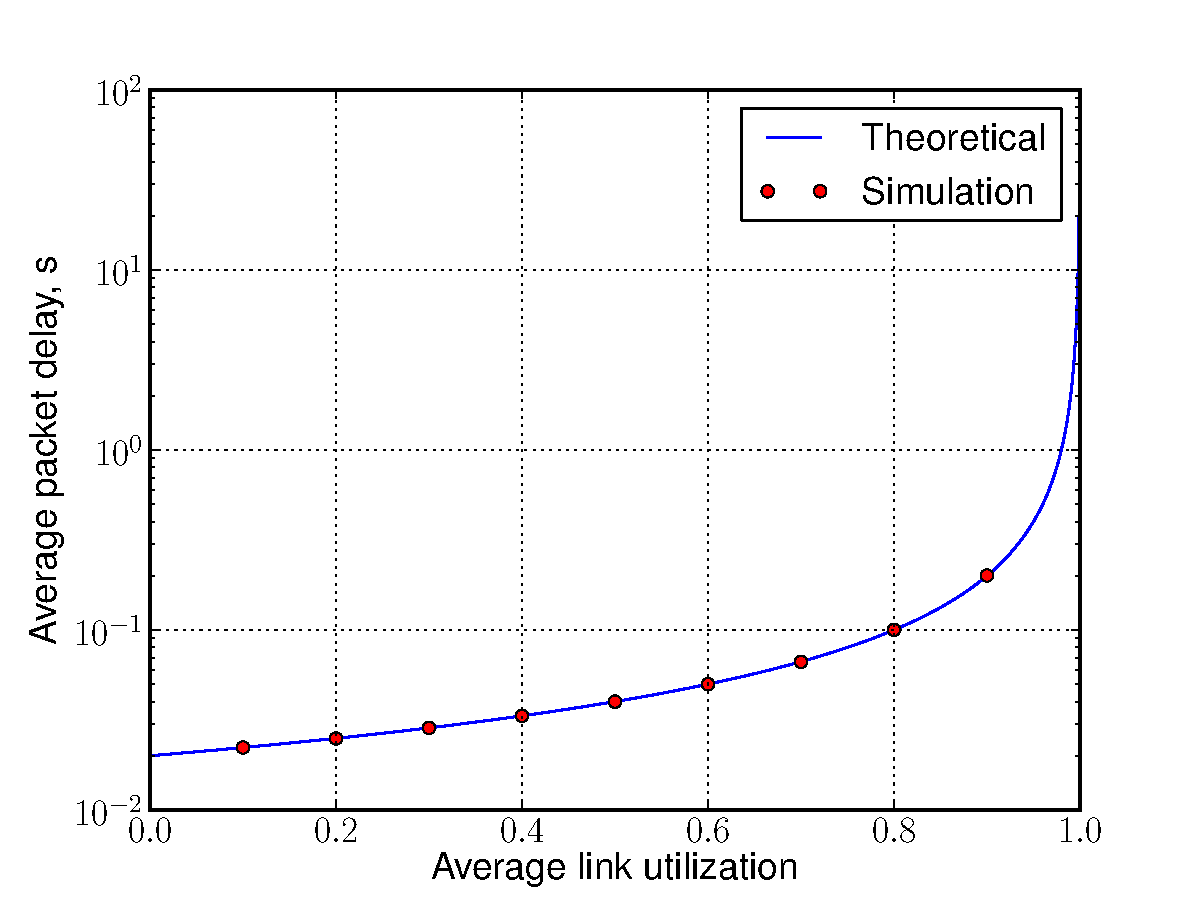
\includegraphics[width=\figsize]{Appendices/Figures/mm1_simulation_results}
	\caption{Comparison of M/M/1 queue simulation results with the theory}
	\label{fig:mm1_simulation_results_simappendix}
\end{figure}

The queueing system was simulated with the following parameters: $\mu=50$ packets per second (pps), and $\lambda\in\{5,10,\ldots,45\}$ pps which is equivalent to $\rho\in\{0.1,0.2,\ldots,0.9\}$. The objective of the simulation was to estimate the steady-state mean packet delay, $T(\rho)$, for each value of the mean link utilization, $\rho$. To this end, for each value of $\rho$, the system was simulated for 1 hour, and a simulation run was replicated 100 times with different seeds to the pseudo-random number generator (PRNG). In all simulation runs, the buffer was initially empty; i.e., there were no packets in the queue. The output of each simulation run constituted a time-series of packet delays in the system. Since the simulation is inherently a nonterminating simulation, the estimation of the steady-state mean packet delay consisted of two steps: 1)~removal of the transient (or warm-up) response of the system, and 2)~averaging within and across the replications with transient response removed. The removal of the transient response was facilitated through the use of the Welch's method~\cite{LawChapter92007}, and for each value of $\rho$, the transient response covered approximately the initial 2000 packet delay samples.

Table~\ref{tab:mm1_simulation_results_simappendix} depicts the estimated steady-state average packet delay for each value of the average link utilization, $\rho$. In all cases, the mean value of the average packet delay closely converges to the theoretical prediction; this conclusion is emphasized in Figure~\ref{fig:mm1_simulation_results_simappendix}. Furthermore, the 95\% confidence interval for the mean of average packet delay does not exceed the factor of $10^{-3}$ for any value of the average link utilization. All in all, this successfully validates the DES simulation engine.

